\documentclass[12pt,titlepage]{article}
\usepackage[ngerman]{babel}
\usepackage[utf8]{inputenc}
\usepackage{color}
\usepackage[a4paper,lmargin={4cm},rmargin={2cm},
tmargin={2.5cm},bmargin = {2.5cm}]{geometry}
\usepackage{amssymb}
\usepackage{amsthm}
\usepackage{graphicx}

\begin{document}

\title{DevOps meets FOSS: Automatisierte Integration von FOSS in die DevOps-Produktentwicklung\\}

\author{Claudia Arnold}

\maketitle

\begin{abstract}
   Unter dem Begriff FOSS bekannt, bietet die Free Open Source Software eine Reihe an Möglichkeiten im Bereich der Softwareentwicklung. Durch die sinkenden Nutzungesbescchränkungen im Vergleich zur konventioneller Software gilt FOSS als ein Instrument zur schnellen Integration von Software in die eigene Entwicklung.  
    \end{abstract}

\section{Einleitung}

\begin{quote}
\textit{In real open source, you have the right to control your own destiny}\newline -Linus Torvalds
\end{quote}

Verändertes Konsumentenverhalten, schnelle Reaktion auf veränderte Kundenwuensche und Time-to-Market sind wesentliche Anforderungen, die für den wirtschaftlichen Erfolg eines Unternehmens insbesondere in Zeiten der Digitalisierung kennzeichnet sind und daher große Herausforderungen mit sich bringen. git staDie daraus resultierenden steigenden Anforderungen an neuer Funktionalität und die damit verbundene stetige Weiterentwicklung erfordern in erster Linie eine neue Dynamik innerhalb der Entwicklug, Konzepte und Tools. In diesem Zusammenhang wird der Softwareentwicklungsprozess nach agilen Methoden unablässig und gehört in den meisten Unternehmen bereits zum Standard einer IT-Organisation. 

In diesem Rahmen kommt der Ansatz des DevOps zum Tragen, nach dessen Grundsätzen der Softwareentwicklungsprozess, angefangen von der Idee, über die schnelle Entwicklung bishin zum Einsatz innerhalb der Produktivumgebung, durchgeführt wird. DevOps ist ein Kofferwort aus den Begriffen Development und IT-Operations und beschreibt im Wesentlichen die technische und organisatorische Verbindung zwischen der Softwareentwicklung und der Systemadministration. Charakterisch sind verkürzte Releasezyklen in einem inkrementellen Prozess und ein hoher Automatisierungsgrad, wodurch eine exakte Planung, Vermeidung von kritischen Fehlern und eine schnelle Reaktion auf Kundenanforderungen ermöglicht wird. Wesentliches Ziel von DevOps ist es, die gesamte Entwicklung transparent, flexibel und agil zu gestalten, wodurch die Produktivität und Effizenz maßgeblich gesteigert und das endgültige Produkt schneller zum Kunden ausgeliefert werden kann. 

Neben der agilen Softwareentwicklung ist ein weiteres wesentliches Kennzeichen des DevOps-Konzeptes die Grundsätze des Lean Manufactoring, nach denen die Minimierung von Verschwendung und die Maximierung der Produktivität im Vordergrund steht. Dabei spielt insbesondere die Wiederverwendung von Software eine wesentliche Rolle. Anstatt einer zeit- und kostenintensiven Neuentwicklung von Software, bleiben viele allgemeine oder wiederholende Funktionalitäten innerhalb eines neuen Projektes oftmals gleich und müssen demnach nicht verändert werden. Vor diesem Hintergrund sparen Entwickler viel Zeit und Ressourcen, indem Quellcode, Templates oder Algorithmen wiederverwendet werden, was wiederrum dem Grundgedanken von DevOps entspricht. 

Ausgehend hiervon ist die Integration von bestehenden Softwarekonzepten ein wesentlicher Vorteil, wodurch die Verwendung von Open Source Software zunehmend an Bedeutung im Unternehmensfeld gewinnt. Als eine realistische Alternative zu herkömlicher Software, erlangte die Open-Source-Bewegung mit der Idee von frei zugänglicher Software in den letzten Jahrzehnten immer mehr an Popularität. Unter Open Source Software versteht man einen öffentlich zugänglichen Quellcode, den jeder einsehen, verändern und für sich nutzen kann. Im Gegensatz zur herkömlicher proprietärer Software, erhalten Nutzer eine Open Source Software meist kostenlos und ohne weitere Kosten für Lizenzvereinbarungen. Durch den unmittelbaren Zugang zum Quellcode, haben Entwickler die Möglichkeit einerseits, am Quellcode mit nur wenigen Ressourcen zu experimentieren und zu überprüfen, ob sich dieser ein wiederkehrendes Problem innerhalb des Projektes beinhaltet oder anderseits nach der jeweligen Problematik zu individualisieren und zu verändern. Die Notwendigkeit einer kosten- und zeitspielige Entwicklung entfällt und die Verwendung von bereits gelösten Paradigmen rückt in den Vordergrund.   

% Häufige Vorgehensweise: Moduale Architektur von Open-Sorce projekten
% Beispiele an OSS aufzeigen: Betriebssysteme, Server-Anwendungen oder Office-Produkte
% Evtl hier nochmal auf Linux, als erstes populäres Produkt im OSS-Bereich eingehen 

Das daraus resultierende Innovationspotenzial kann, basierend auf der freien Gestaltungsfreiheit die OSS im Gegensatz zur kommentieller Lizenzsoftware ermöglicht, genutzt werden, Ideen umzusetzen ohne zu stark an unternehmensinterne Vorgaben gebunden zu sein oder unternehmensinterne Prozesse oder Prozessabläufe in die Entwicklung einzubinden. Vor diesem Hintergrund kann eine umfassende Integration von Open Source Software in vorhandene Unternehmenstrukturen im Bereich der Entwicklung, ausschließlich in einem agilen Umfeld durchgeführt werden, womit DevOps als ideale Plattform geeignet ist.  

Trotz der Freiheiten, die Open Source Software offensichtlich bietet, unterliegen die meisten Projekte rechtlichen Schutzmaßnahmen, einschließlich dem Marken- Patent- und Urheberrecht. Aufgrund dessen können, aus der Verwendung von OSS resultierende Lizenzfragen oder rechtliche Konsequenzen, zu einer maßgeblichen Einschränkung insbesondere im Hinblick auf eine mögliche Verteilung oder Weitergabe an Dritte führen, die von Unternehmen genau analysiert und überprüft werden muss.  

In dieser Thesis werden die grundsätzlichen Vorteile und Risiken, die sich aus den verschiedenen Lizenzvereinbarungen bei der Verwendung von OSS ergeben analysiert und die Migration in den Devops-Emntwicklungsprozeess dargestellt. Verdeutlicht wird die Themenstellung anhand der ausgeführten Analysen anahnd eines Beispiels bei der msg Systems. 




Durch die freie Verfügbarkeit des Quellcodes, die entfallenen Lizenzkosten für den Einsatz und die freie Weiterentwicklungsmöglichkeiten, erweist sich OSS als eine einfache und kostengünstige Innovationsquelle für Unternehmen. 

Dabei reicht das Anwendungsfeld für die Verwendung von OSS in diesem Zusammenhang von der Automobilindustrie bis zur Versicherungsbranche und steht daher im direkten Wettbewerb zu proprietären Softwareangeboten. 

\subsection{Problemstellung}

Wie bereits beschrieben unterliegen 





In diesem Abschnitt wird beschrieben, welche derzeitige Problemstellung innerhalb der DevOps Produktentwicklung bei der Integration von FOSS vorliegt, die mittels der Thesis gelöst bzw verbessert werden kann. Insbesondere wird dabei auf die derzeitige Ist-Situation eingegangen, welche Herausforderungen momentan vorliegen (bei msg und allgemein) und wie der aktuelle Stand der Wissenschaft in diesem Kontext ist. 
Zudem wird eine Herleitung zu den Ziel und den Forschungsfragen dieser Thesis hergestellt.  

\subsection{Ziel und Fragestellung}

Unter diesen Gesichtspunkten lassen sich fünf Forschungsfragen für diese Arbeit wie folgt ableiten:\\ 

1. Welche praxisrelevanten Informationen können aus OSS extrahiert und verwendet werden?\\ 

%(Lizenzmodelle)
% was soll die Zielgruppe dieser Frage sein? --> Mehrheitlich die Devops-Umgebung (dh. Entwickler, Softwaredienstleister)
% zunächst grundlegende Informationen aufzuzeigen, danach den praxisrelevanten Kontext beachten (Überblick schaffen)


2. Welche Einschränkungen sind bei der Verwendung von OSS in Hinblick auf die verschiedenen Lizenzinformationen zu berücksichtigen?\\ 

%(Haftungs-/Garantiebedingungen, Autorenhinweise, Copyleft-Bedinungen)
%Anhand von praxisrelevaten Lizemzmodellen, werden ausschließlich diese mit Einschränkungen versehen, die anderen eher erwähnen. 
%Praxisrelevanz wird anhand des beschriebenen Produktes bei msg festgelegt


3. Welche prozessualen Anpassungen müssen anhand der gewonnenen Erkenntnisse getroffen werden, um auf mögliche Veränderungen in den Lizenzinformationen reaktionsschnell vorbereitet zu sein?\\ 

% GEnerell HAF-Projekt verwenden, kein exaktes Produkt da der Entwicklungspriozess gleich abläuft. 
% Ist-zustand muss exakt dargestellt werden, (Manuelle Aktualsierung aller FOSS-BEdinugngen und Deklarationen erforderlich) + gängiger Prozess muss designt werden!
% Ist-Zustand: OSS wird genommen und modifiziert und im Rahmen der Unternehmung ausgeliefert 
% --> Daraus ergibt sich der Soll- Zustand, indem die Einschränkungen basierend auf Frage 2, zum Tragen kommen und die Situationen aufzeigen, in dem sich der Ist-Zustand verändern muss --> Veränderungen am Prozessmodell angepasst 
% Welche Stakeholder sind beteiligt, wer hat welche Verantwortung/Pflichten/Aufgaben --> welche Informationen müssen weitergegeben werden
%Hieraus ergeben sich je nach beteiligten Stakeholder, unterschiedliche Verantwortungen, Pflichten und Aufgabengebiete.





%% (evtl.) Proof of Concept
%Prozess wird dargestellt --> Wie wird dieser durchgeführt/Wie wird erreicht?


4. Wie können relevante Lizenzinformationen und haftungsbedingte Anforderungen anhand eines Produktes automatisiert aus den verwendeten Lizenzmodellen aus OSS herausgearbeitet werden?\\ 

%(Programm, Makros ???)\\
%Soll-Prozess wird implentiert --> Konkrektes Beispiel
%Automasierungsgrad muss hoch sein, in Sinne von Devops


5. Wie kann die Transparenz der gesammelten Informationen insgesamt sichergestellt werden?\\ 

%(Wie kommen die Informationen schnell an das Devops-Team)\\ 
%Transparenz/Kommunikation muss gewährleistet werden --> Änderungen des Lizenzkonstellation muss tranzparent gestaltet werden (zb. Dashboards, Alters, REports)
%Dokumentation  

Ziel dieser Arbeit ist es, zunächst Informationen im Bereich DevOps und OSS zu gewinnen und dabei insbesondere die Einschränkungen der unterschiedlichen Lizenzmodelle zu beschreiben. Hierzu wird insbesondere auf die juristischen Regelungen der OS-Linzenzen und die rechtlichen Konsequenzen bei einem Nichteinhalten der gesetzlichen Schutzmaßnahmen, die sich für ein Unternehmen ergeben kann, näher eingegangen. In diesem Zuge werden prozessuale Anpassungen im DevOps-Prozess vorgenommen, die sich einerseits durch die Auslieferung des Softwareproduktes nach der Modifikation von OSS oder anderseits durch Änderungen von Lizenzbestimmungen während des Softwareentwicklungsprozesses ergeben. Ausgehend von den prozessualen Veränderung soll innerhalb der praxisorientierten Umsetzung, eine Möglichkeit dargestellt werden, wie die gewonnenen Ergebnisse automatisiert herausgearbeitet werden und der Informationsfluss innerhalb des ganzen DevOps-Teams sichergestellt werden kann.
 

\subsection{Aufbau dieser Arbeit}

Der Aufbau dieser Arbeit ist in fünf wesentliche Kapitel unterteilt. Zunächst wird auf den theoretischen Hintergrund von DevOps und OSS eingegangen. Der theoretische Teil von DevOps fokussiert auf die Grundlagen und die Funktionsweise. Innerhalb der OSS-Theorie wird insbesondere auf die Grundlagen, Lizenzbedingungen anhand des Copyleft-Effekts und den rechtlichen Gesichtspunkt näher eingangen. Das dritte Kapitel fokussiert sich, auf die Anpassung des Softwareentwicklungsprozesses durch den Einsatz von OSS auf Basis der gewonnenen Informationen. Darüber hinaus wird eine manuelle Checkliste, für den präventiven Gebrauch vorgestellt. In Kapitel vier wird die Realisierbarkeit und Machbarkeit der erhobenen Konzepte anhand eines Proof of Concept dargestellt. In Kapitel fünf folgt eine Schlussfolgerung und ein entsprechender Ausblick. 

\section{Fachlicher Rahmen}

In diesem Abschnitt werden grundlegende Prinzipien zu DevOps und FOSS dargetellt, um damit das Verständnis der Leser zu stärken.\\

\begin{figure}[h]
    \centering
    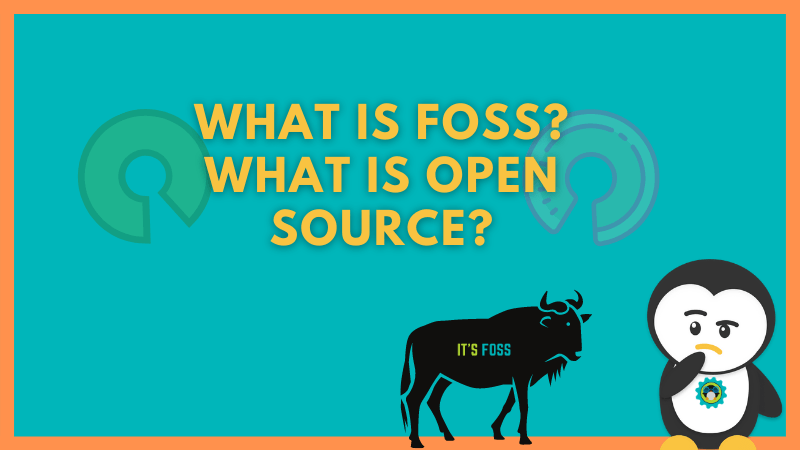
\includegraphics[scale=0.7]{Bilder/what-is-foss}
    \caption{Ein Beispiel}
\end{figure}

\subsection{DevOps}

Anhand des DevOps-Ansatzes wird eine Kultur oder Umgebung etabliert, durch die das Erstellen, Testen und Freigeben von Software schnell, häufig und zuverlässiger erfolgen kann. \cite[S.xxviii]{sharma_devops_2017} Obwohl die Gründe für die Einführung von DevOps vielschichtig sein können, sollen in erster Linie Ineffizienzen in den Softwareentwicklungs-, Release- und Betriebsprozessen vermieden werden, die durch die organisatorische Trennung zwischen den Prozessen \cite{lwakatare_devops_2019} oder durch die Fehlkommunikation zwischen den Teammitgliedern \cite{ebert_devops_2016} verursacht werden. Generell ist es für Teams innerhalb der Entwicklung nicht möglich, neue Softwareversionen freizugeben oder Softwareänderungen schnell vorzunehmen, wenn der Betrieb die jeweiligen Funktionen nur langsam bereitstellen kann. \cite[S. 7,8]{sharma_devops_2017} Vor diesem Hintergrund stehen die Bereiche der Entwicklung und des Betriebs oft im Zielkonflikt "Agilität vs. Stabilität" und sehen sich mit verschiedenen Hindernissen konfrontiert, darunter unbefriedigende Testumgebungen und schlechter Informationsfluss. \cite{lwakatare_devops_2019}, \cite[S. 8]{sharma_devops_2017}, \cite{konig_devopswelcome_2019} Die Folgen sind eine verspätete Bereitstellung von Releases, Fehler in den Releases oder eine fehlende Dokumentation. \cite[S. 24]{alt_innovationsorientiertes_2017} Hinzu kommen Probleme wie mangelndes Knowhow von Entwicklen über die Betriebnahme der verwendeten Systeme, fehlendes Vertrauen in den Ops-Bereich hinsichtlich der Stabilität, verzögertes Testen oder Verschwendung durch mangelnde Wiederverwendung von Quellcode. \cite{humble_why_2011}\\\\ Mittels DevOps sollen die Interessen aller Beteiligten ausglichen werden, mit besonderem Schwerpunkt auf Entwicklern, Testern und Betriebspersonal. \cite{humble_why_2011} Die querschnittlich aufgestellten Teams, lösen sich aus abgegrenzten Organisationseinheiten und Verantwortungsbreichen, aus den sogenannten 'Silos' und treiben gemeinsame Ergebnisse durch eine effektive Zusammenarbeit voran. \cite[S.5]{halstenberg_devops_2020}, \cite{sollner_devops_2017} Die daraus resultierenden Vorteile, reichen von einer schnelleren Produktbereitstellung, bessere Ressourcenauslastung und Automatisierung bishin zu einer stabileren Betriebsumgebung. 

\paragraph{2.1.3.1 CALMS} $~$
Generell lassen sich die Werte von DevOps, wie in Abbildung 2 dargestellt, in dem bekannten Akronym CALMS zusammenfassen: Kultur (Culture), Automatisierung (Automation), Schlankheit (Lean), Messung (Measurement) und Teilen (Sharing). 

\begin{figure}[h]
     \centering
     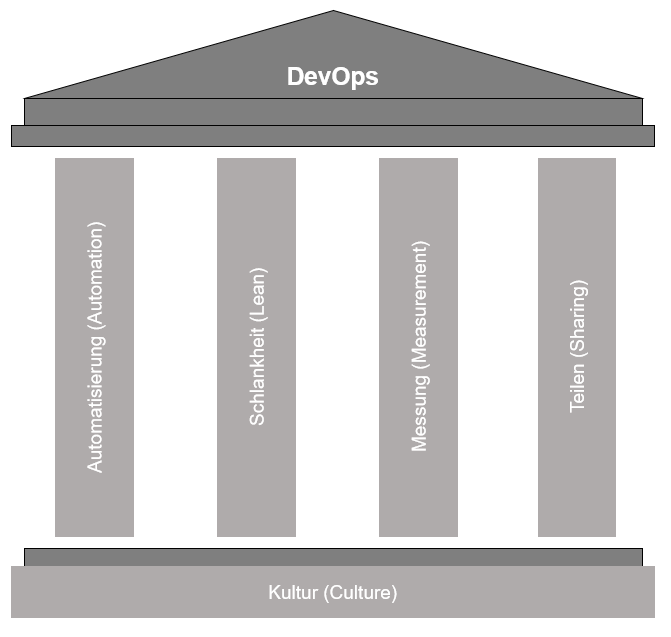
\includegraphics[scale=0.4]{Bilder/Calms.png}
     \caption{Die Säulen von DevOps, basierend auf dem CALMS-Prinzip, angelehnt an \cite{hornby_devops_nodate}}
 \end{figure}

Der Aspekt der Kultur beinhaltet zunächst die Ausrichtung nach dem Menschen. Hierbei spielt die Kollaboration als ein funktionsübergreifendes Team und die Orientierung nach Kundenwünschen eine tragende Rolle für eine DevOps-Organisation. \cite[S.5]{halstenberg_devops_2020} Die Automatisierung von Entwicklung, Implementierung und Tests ist der Schlüssel zum Erreichen niedriger Vorlaufzeiten und damit zu schnellem Feedback. \cite{humble_why_2011} 'Lean' steht in diesem Zusammenhang für die Vermeidung von Verschwendung jedlicher Ressourcen, Transparenz, ganzheitliche Betrachtung und Prozessoptimierung. Der Faktor der Messung orientiert sich an den messbaren Daten, um den Fortschritt eines Unternehmens zu begutachten. Die definierten und erhobenen Kennzahlen reichen dabei von den Verfügbarkeiten und den Zeiten für die Fehlerbehebung oder Codeänderungen bis zu den Zeiten für die Anforderungsänderungen. \cite[S. 7]{halstenberg_devops_2020} Die letzte Säule beschreibt das Teilen von Informationen, Wissen, Vorgehensweisen und Praktiken innerhalb eines oder zwischen verschiedenen Teams unterschiedlicher Abteilungen. \cite{halstenberg_devops_2020} Dabei soll eine Umgebung geschaffen werden, in der gegenseitige Austausch, die Kommunikation und die gemeinsame Nutzung im Vordergrund stehen.\\\\

Bei dem gesamten Vorteilen und Mehrwerten, die durch DevOps erreicht werden können, kann DevOps jedoch als kein Nullsummenspiel oder Selbstläufer gesehen werden. \cite{humble_why_2011} Der DevOps-Ansatz benötigt zunächst einen kulturellen Wandel, was eine große Herausforderung für viele Unternehmen darstellen kann. Standardisierte Herangehensweisen sind von einer Vielzahl von Unternehmen über die Jahre tiefgreifend verankert worden, wodurch Mitarbeiter ihre gewohnten Arbeitsabläufe anpassen müssten. Dies reicht von der Erlernung neuer Tools, Technologien und Methoden, Aufbau einer Kommunikation für den gegenseitigen Austausch, vollständige Automatisierung, Verschmelzung etablierter Rollen und Zuständigkeiten, Schwierigkeiten bei der Implementierung eines automatisierten Deployment-Prozesses oder die Übernahme neuer Aufgaben und Verantworlichkeiten. \cite{lwakatare_devops_2019}, \cite[S. 594 - 595]{abrahamsson_product-focused_2016}, \cite[S. 43 - 45]{halstenberg_devops_2020} Da sich die Bedeutung von DevOps in den letzten Jahren verschoben hat und immer wieder neue Tools für DevOps auftauchen, handelt es sich bei DevOps um eine stetige Weiterentwicklung. \cite[S. 595]{abrahamsson_product-focused_2016} Daher gibt es keinen Standard fester Praktiken im Zusammenhang mit DevOps, wodurch sich nicht festlegen lässt, welche Praktiken für DevOps eingesetzt werden sollten. 


% Insgesamt soll das Ziel verfolgt werden, die Softwarebereitstellung kontinuierlich sicherzustellen um so reaktionschnell auf Veränderungen am Markt oder Kundenanforderungen reagieren zu können.

%Die Trennung zwischen Projekten und Betrieb ist zu einer schwerwiegenden Einschränkung geworden, einerseits für die Fähigkeit von Unternehmen, neue Funktionen schneller auf den Markt zu bringen, andererseits für die der IT, stabile und qualitativ hochwertige Systeme und Dienste zu warten. \cite{humble_why_2011} 

%Ersetzen von Softwareentwicklungsmethode durch Kultur, Bewegung oder Praxis.
%Hinzufügung des Hinweises auf Automatisierung

%In diesem Abschnitt werden die grundsächlichen Merkmale von Devops beschrieben. Zudem werden wesentliche Vorteile beschrieben, durch die die Integration von DevOps möglich sind. Des weiteren wird auf das CALMS-Modell (Culture, Automation, Lean, Measurement und Sharing) eingegangen.

%DevOps gilt nicht als ein Nullsummenspiel, indem die Bereitstellungen häufig und zuverlässig in einer stabilen Produktumgebung erreicht werden, sondern es ist ein Ansatz zur Behebung der genannten Probleme durch Kultur, Automatisierung, Schlankheit, Messung und gemeinsame Nutzung, welches auch als CALMS bekannt ist. \cite{humble_why_2011



% Die Abbildung 2 zeigt den chronischen Konflikt, der oftmals innerhalb der IT-Organsisation herrscht, der durch fehlende Interaktion zwischen diesen Bereichen enstehen, die häufig unterschiedliche Ziele und Prozesse verfolgen. \cite[S. 349 - 350]{kim_devops-handbuch_2017}

% \begin{figure}[h]
%     \centering
%     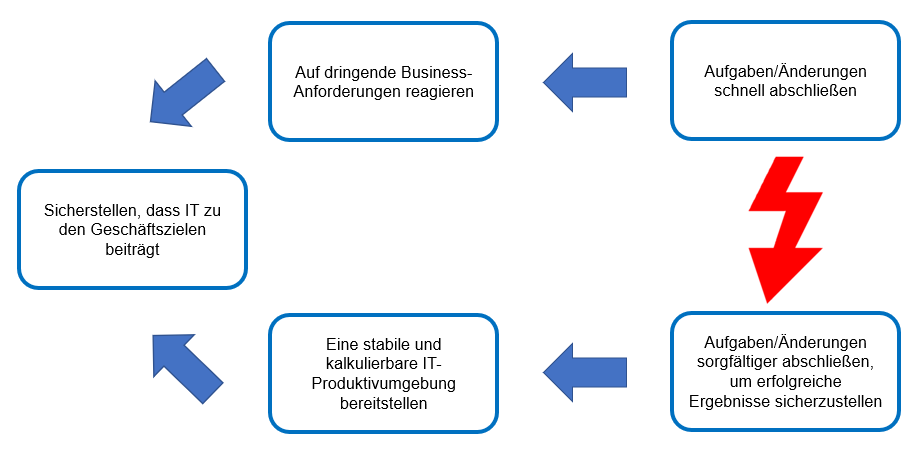
\includegraphics[scale=0.6]{Bilder/Core Conflict Clouds}
%     \caption{Zentraler chronischer Konflikt nach Gene Kim \cite[S. 349]{kim_devops-handbuch_2017}}
% \end{figure}
% \dwi{irgendwie hab ich das gefühl diese grafik "läuft" in die falsche richtung.}

\subsubsection{Was ist DevOps?}
\subsubsection{DevOps-Kultur}
\subsubsection{DevOps-Lifecycle}
\subsubsection{Softwareauslieferungen}
\subsubsection{Automatisierung}
\subsubsection{IaaS}
\subsubsection{Herausforderungen/Nachteile}


\subsection{FOSS}

\centering
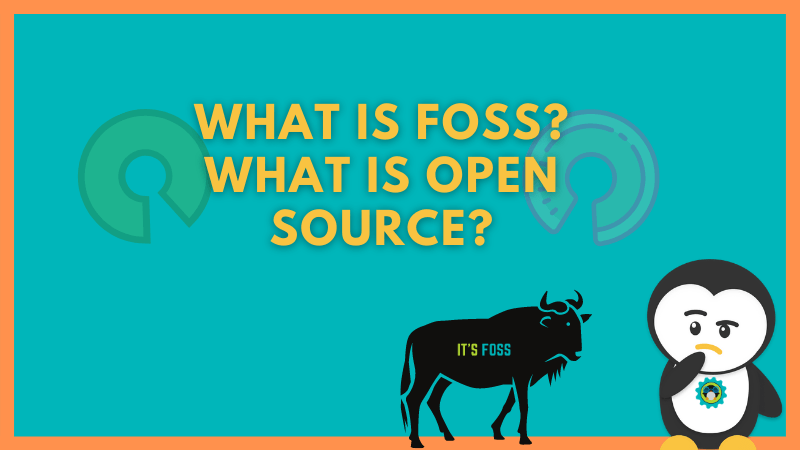
\includegraphics[scale=0.7]{Bilder/what-is-foss}

\section{Proof of Concept}

Während die manuelle Checkliste dafür verwendet wird, präventiv OSS-Komponenten mit riskanten Lieznzmodellen bereits zu Beginn des Entwicklungsprozesses zu vermeiden, soll die automatisierte Checkliste das Ziel verfolgen, bereits implementierte OSS-Komponenten auf ihre Lizenzmodelle zu prüfen, bevor diese ausgeliefert werden. 

Diese wird innerhalb des folgenden Kapitels als der Proof of Concept (PoC) näher beschrieben. 

Grundsätzlich bestimmt der PoC die Machtbarkeit einer Idee, also ob die Idee wie geplant funktioniert und in die Realität umgesetzt werden kann, bevor für diese Ressourcen auf Produktionsebene verschwendet werden.  

In dem Rahmen dieser Arbeit stellt der PoC einen Prototypen dar, der die prinzipelle Durchführbarkeit einer automatisierten Checkliste aufzeigt, wobei dieser nicht direkt innerhalb des Build-Prozess integriert sondern unabhängig von dem jetzigen Entwicklungsprozess entwickelt wurde.  

Obwohl der PoC nicht immer mit einem Prototypen gleichzusetzten ist, werden in diesem Fall beide Begriffe gleichermaßen behandelt. 

Die automatisierte Checkliste soll dabei als eine reduzierte Version des Endprodukts umgesetzt werden, die auf ihre Nutzbarkeit und Funktionalität getestet und bewertet werden kann. 

Hierbei wird der Prototyp nicht alle Merkmale und Funktionen eines marktreifen Produkts aufweisen, allerdings wird einerseits die generelle Nutzbarkeit in Abhängigkeit der bestehenden Systemumgebung und andererseits die Demonstration der entwickelten Funktionalitäten zum Zweck einer generellen Realisierbarkeit aufgezeigt. 

Gleichzeitig dient der PoC als eine Basis für weitere Weiterentwicklungsmöglichkeiten. 

Da die direkte Entwicklung innerhalb eines aktiven Projekts große Herausforderungen und Probleme mit sich bringen kann, wurde der Prototyp mit den Kollegen des Projektes bei der msg systems ag, ausgearbeitet und innerhalb dieser Arbeit festgehalten. 

Dies hatte den Vorteil, dass unvorhersehbare Problemfelder berücksichtigt wurden und der Prototyp direkt in die Systemlandschaft eingebunden werden konnte, ohne den gesamten Projektablauf in Mitleidenschaft zu ziehen.

Der PoC wurde mit der Skizzierung der grundsätzlichen Idee begonnen. 

Wesentliche Elemente waren hierbei die momentane Problembeschreibung als auch die darauf aufbauende Lösung, die umgesetzt werden soll. 

Die Ausarbeitung als auch der Umfang des zugrundeliegenden Problems wurden zunächst durch die Gespräche mit mehreren Teammitgliedern und durch die Teilnahme an Teammeetings anfänglich skizziert.

In diesem Rahmen wurde \textit{die fehlende Bewertung und Prüfung bei der Verwendung von OSS} als das wesentliche Problem identifiziert, welches mithilfe einer automatisierten Überprüfung gelöst werden sollte.  

Demnach sollte der Protoytyp verwendete OSS-Komponenten anhand ihrer Lizenzmodelle analysieren und bei einem, mit Risiko verbundenen Lizenzmodell, den jeweiligen Entwickler darüber zeitnah in Kenntnis setzen.  

Die weitere Anforderungsdefinition, Gestaltung und Einbeziehung erfolgte im Zuge der Prozessmodellierung und der dazugehörigen Anpassung des Soll-Prozesses und wurde in vier grundlegende Schritte unterteilt.





\end{document}

